\documentclass[12pt]{article}
\newif\ifblind
\blindfalse % The Journal of Economic Psychology does not admit anonymized submissions
% Bibliography: Elsevier author-year style (instead of the style of the common preamble), without page back-references
\let\joeporiginalbibliographystyle\bibliographystyle
\renewcommand{\bibliographystyle}[1]{} % ignore the style set in preamble_paper.tex
% Common preamble of wellbeing.tex, wellbeing_region.tex and wellbeing_discrepancy.tex
% Compile from papers/:  latexmk -pdf -outdir=build <file>.tex
\usepackage[T1]{fontenc}
\usepackage[utf8]{inputenc}
\usepackage{tgpagella}
\usepackage{mathpazo}
\usepackage[margin=1in]{geometry}
% \linespread{2}
% \usepackage[super,comma,sort]{natbib} % WPcomment
\usepackage[round,sort&compress]{natbib} % NCCcomment
% \usepackage[natbibapa]{apacite}
% \bibliographystyle{apacite} 
\usepackage{url} % [hyphens]
\usepackage{tcolorbox}
\usepackage{xr-hyper} % cross-references between the main paper and its Online Appendix (must be loaded before hyperref)
\usepackage[hyperpageref]{backref} % back references biblio. Needs latexmk at compilation. Incompatible with apacite.
% \usepackage{hyperref}
\usepackage[pagebackref]{hyperref} % Incompatible with apacite.
% \usepackage{hyperref}
% \usepackage{multibib} % incompatible with backref
\hypersetup{
  colorlinks=true, % breaklinks=true,
  urlcolor=purple,    % color of external links
  linkcolor=blue,  % color of toc, list of figs etc.
  citecolor=violet,   % color of links to bibliography
}
\usepackage{setspace}
\onehalfspacing
\usepackage{amsmath, amssymb}
\usepackage{graphicx}
\usepackage{booktabs, makecell, threeparttable, adjustbox}
\usepackage{caption}
\captionsetup{font=small, labelfont=bf}
\ifblind
  \bibliographystyle{plainnat}
\else
  \bibliographystyle{plainnaturl_clean}
\fi
\usepackage{xspace}
\xspaceaddexceptions{]\%} % no space inserted by \xspace before "]" or "\%" (e.g. after number macros)
\usepackage{xcolor}
\usepackage{lineno}
% Placeholders for information to be completed by the author
\newcommand{\todo}[1]{\textcolor{red}{[TODO: #1]}}
% Numbers computed by code_wellbeing/main.R (percentages are given without the % sign)
\newcommand{\nEVSSurveys}{36\xspace}
\newcommand{\nNewWVSSurveys}{2\xspace}
\newcommand{\nEVSSameYearWVS}{3\xspace}
\newcommand{\nEVSvsWVS}{10\xspace}
\newcommand{\meanAbsDiffEVSWVS}{0.28\xspace}
\newcommand{\maxAbsDiffEVSWVS}{0.53\xspace}
\newcommand{\corGallupWHR}{0.993\xspace}
\newcommand{\corGallupWHRoldMapping}{0.89\xspace}
\newcommand{\nGallupCountryYears}{2,351\xspace}
\newcommand{\nGallupCountries}{168\xspace}
\newcommand{\nWVSCountryYears}{342\xspace}
\newcommand{\nWVSCountries}{112\xspace}
\newcommand{\nWVSRespondents}{501,911\xspace}
\newcommand{\nFabre}{11,000\xspace}
\newcommand{\nFabreCountries}{10\xspace}
\newcommand{\shareRegionBetterNoLatam}{70\xspace}
\newcommand{\shareRegionBetterNoEE}{73\xspace}
\newcommand{\shareRegionBetterSixRegions}{100\xspace}
\newcommand{\shareRegionBetterUN}{100\xspace}
\newcommand{\bestIncome}{Cluster k=7 nominal\xspace}
\newcommand{\shareRegionBetterWVS}{88\xspace}
\newcommand{\shareRegionBetterWVSbest}{79\xspace}
\newcommand{\nSpecsWVS}{952\xspace}
\newcommand{\meanShareIncomeBest}{33\xspace}
\newcommand{\meanRtwoIncomeBest}{20\xspace}
\newcommand{\meanRtwoIncomePPP}{14\xspace}
\newcommand{\meanRtwoRegion}{33\xspace}
\newcommand{\RtwoSatisfiedMeanPPP}{23\xspace}
\newcommand{\RtwoHappinessMeanPPP}{4\xspace}
\newcommand{\RtwoVeryHappyPPP}{0\xspace}
\newcommand{\shareRegionBetterGallup}{34\xspace}
\newcommand{\shareIncomeGallupMean}{60\xspace}
\newcommand{\RtwoGallupMeanPPP}{61\xspace}
\newcommand{\RtwoGallupRegion}{48\xspace}
\newcommand{\RtwoWHRPPP}{63\xspace}
\newcommand{\RtwoWHRRegion}{55\xspace}
\newcommand{\shareRegionBetterWVSonly}{100\xspace}
\newcommand{\shareRegionBetterNoLatamEE}{27\xspace}
\newcommand{\shareIncomeNoLatamEE}{35\xspace}
\newcommand{\shareRegionBetterContinents}{48\xspace}
\newcommand{\shareRegionBetterContinentsFive}{48\xspace}
\newcommand{\shareRegionBetterContinentsSixOld}{48\xspace}
\newcommand{\shareRegionBetterWB}{55\xspace}
\newcommand{\cvIncomeSatisfiedMean}{0.21\xspace}
\newcommand{\cvIncomeBestSatisfiedMean}{0.23\xspace}
\newcommand{\cvRegionSatisfiedMean}{0.37\xspace}
\newcommand{\cvIncomeGallupMean}{0.60\xspace}
\newcommand{\cvRegionGallupMean}{0.45\xspace}
\newcommand{\shareCvRegionBetterWVS}{100\xspace}
\newcommand{\ciLowWVSMeanRIncome}{9\xspace}
\newcommand{\ciHighWVSMeanRIncome}{20\xspace}
\newcommand{\ciLowWVSMeanRRegion}{26\xspace}
\newcommand{\ciHighWVSMeanRRegion}{42\xspace}
\newcommand{\ciLowWVSMeanShare}{16\xspace}
\newcommand{\ciHighWVSMeanShare}{32\xspace}
\newcommand{\ciLowWVSRIncome}{14\xspace}
\newcommand{\ciHighWVSRIncome}{34\xspace}
\newcommand{\ciLowWVSRRegion}{30\xspace}
\newcommand{\ciHighWVSRRegion}{52\xspace}
\newcommand{\ciLowWVSShare}{21\xspace}
\newcommand{\ciHighWVSShare}{45\xspace}
\newcommand{\ciLowGallupRIncome}{52\xspace}
\newcommand{\ciHighGallupRIncome}{69\xspace}
\newcommand{\ciLowGallupRRegion}{38\xspace}
\newcommand{\ciHighGallupRRegion}{61\xspace}
\newcommand{\ciLowGallupShare}{49\xspace}
\newcommand{\ciHighGallupShare}{68\xspace}
\newcommand{\meanShareIncomePPP}{23\xspace}
\newcommand{\corHappySatisfied}{0.72\xspace}
\newcommand{\corHappinessSatisfactionMean}{0.75\xspace}
\newcommand{\corVeryHappySatisfiedMean}{0.60\xspace}
\newcommand{\slopeVeryHappy}{0.002\xspace}
\newcommand{\pVeryHappy}{= .948\xspace}
\newcommand{\happiestFirst}{Switzerland\xspace}
\newcommand{\happiestFirstN}{10\xspace}
\newcommand{\happiestSecond}{Mexico\xspace}
\newcommand{\happiestSecondN}{9\xspace}
\newcommand{\happiestThird}{Kyrgyzstan\xspace}
\newcommand{\happiestThirdN}{6\xspace}
\newcommand{\happiestRegionWestern}{25\xspace}
\newcommand{\happiestRegionLatinAmerica}{19\xspace}
\newcommand{\happiestRegionAsia}{15\xspace}
\newcommand{\happiestRegionAfrica}{5\xspace}
\newcommand{\nHappiestCells}{64\xspace}
\newcommand{\happiestAllWavesTop}{Kyrgyzstan 2020 (3 indicators, including mean happiness)\xspace}
\newcommand{\happiestAllWavesOthers}{Finland 1981, Malaysia 2012, Mexico 2012, Qatar 2010 and Vietnam 2020\xspace}
\newcommand{\happiestAllWaves}{Kyrgyzstan--2020 (3 indicators: Very Happy, V. Happy -- V. Unhappy, Happiness (mean)); Finland--1981 (Satisfied); Malaysia--2012 (Very Unhappy); Mexico--2012 (Satisfaction (mean)); Qatar--2010 (Happy); Vietnam--2020 (Happy + Satisfied)\xspace}
\newcommand{\treeRegionFirst}{8\xspace}
\newcommand{\withinRtwoSatisfiedMean}{0.34\xspace}
\newcommand{\meanWithinRtwo}{0.24\xspace}
\newcommand{\withinSlopeSatisfiedMean}{2.31\xspace}
\newcommand{\crossSlopeSatisfiedMean}{1.14\xspace}
\newcommand{\withinSlopeVeryHappy}{0.21\xspace}
\newcommand{\pWithinVeryHappy}{< .001\xspace}
\newcommand{\nWithin}{312\xspace}
\newcommand{\RtwoFreedomSatisfaction}{63\xspace}
\newcommand{\shapleyFreedom}{42\xspace}
\newcommand{\shapleyFreedomRegion}{21\xspace}
\newcommand{\shapleyFreedomIncome}{11\xspace}
\newcommand{\RtwoTolerance}{24\xspace}
\newcommand{\RtwoGod}{1\xspace}
\newcommand{\RtwoGrowth}{2\xspace}
\newcommand{\RtwoMedianIncome}{19\xspace}
\newcommand{\shapleyMedianIncome}{7\xspace}
\newcommand{\shapleyMedianIncomeIncome}{11\xspace}
\newcommand{\shapleyMedianIncomeRegion}{32\xspace}
\newcommand{\nMedianIncome}{339\xspace}
\newcommand{\RtwoHFCE}{30\xspace}
\newcommand{\shapleyHFCE}{13\xspace}
\newcommand{\shapleyHFCEIncome}{10\xspace}
\newcommand{\shapleyHFCERegion}{29\xspace}
\newcommand{\nHFCE}{292\xspace}
\newcommand{\RtwoGDPMedianSample}{23\xspace}
\newcommand{\deatonGrowth}{\ensuremath{-}5.50\xspace}
\newcommand{\deatonGrowthSe}{2.28\xspace}
\newcommand{\pDeatonGrowth}{= .017\xspace}
\newcommand{\deatonIncome}{0.80\xspace}
\newcommand{\nDeaton}{120\xspace}
\newcommand{\deatonGrowthNoExCommunist}{\ensuremath{-}0.53\xspace}
\newcommand{\deatonGrowthSeNoExCommunist}{2.89\xspace}
\newcommand{\pDeatonGrowthNoExCommunist}{= .855\xspace}
\newcommand{\deatonIncomeNoExCommunist}{0.86\xspace}
\newcommand{\nDeatonNoExCommunist}{93\xspace}
\newcommand{\growthCoefWVS}{0.039\xspace}
\newcommand{\growthSeWVS}{0.019\xspace}
\newcommand{\pGrowthWVS}{= .044\xspace}
\newcommand{\growthCoefGallup}{0.001\xspace}
\newcommand{\growthSeGallup}{0.010\xspace}
\newcommand{\pGrowthGallup}{= .957\xspace}
\newcommand{\nonresponseSatisfactionWVS}{1.4\xspace}
\newcommand{\nonresponseHappinessWVS}{1.7\xspace}
\newcommand{\corNonresponseGDP}{\ensuremath{-}0.09\xspace}
\newcommand{\veryHappyKGZ}{68\xspace}
\newcommand{\satisfactionKGZ}{8.4\xspace}
\newcommand{\gdpKGZ}{5,500\xspace}
\newcommand{\maxVeryHappyIsKGZ}{1\xspace}
\newcommand{\veryUnhappyEGY}{42\xspace}
\newcommand{\effectLadder}{\ensuremath{-}0.45\xspace}
\newcommand{\seLadder}{0.05\xspace}
\newcommand{\effectScale}{0.14\xspace}
\newcommand{\seScale}{0.05\xspace}
\newcommand{\effectLadderZeroTen}{\ensuremath{-}0.46\xspace}
\newcommand{\effectScaleZeroTen}{\ensuremath{-}0.26\xspace}
\newcommand{\effectLadderSatisfied}{\ensuremath{-}9\xspace}
\newcommand{\interactionLadderIncome}{\ensuremath{-}0.004\xspace}
\newcommand{\pInteractionLadderIncome}{= .919\xspace}
\newcommand{\ciLowInteractionLadderIncome}{\ensuremath{-}0.086\xspace}
\newcommand{\ciHighInteractionLadderIncome}{0.077\xspace}
\newcommand{\interactionLadderScale}{0.008\xspace}
\newcommand{\seInteractionLadderScale}{0.092\xspace}
\newcommand{\pInteractionLadderScale}{= .930\xspace}
\newcommand{\gradientIncomeSatisfaction}{0.69\xspace}
\newcommand{\tripleInteraction}{\ensuremath{-}0.023\xspace}
\newcommand{\pTripleInteraction}{= .786\xspace}
\newcommand{\interactionLadderIncomeFull}{0.009\xspace}
\newcommand{\pInteractionLadderIncomeFull}{= .883\xspace}
\newcommand{\interactionScaleIncome}{0.106\xspace}
\newcommand{\pInteractionScaleIncome}{= .083\xspace}
\newcommand{\pHeterogeneityWording}{< .001\xspace}
\newcommand{\chiHeterogeneityWording}{93.4\xspace}
\newcommand{\wordingCHE}{\ensuremath{-}0.34\xspace}
\newcommand{\wordingDEU}{\ensuremath{-}0.53\xspace}
\newcommand{\wordingESP}{\ensuremath{-}1.12\xspace}
\newcommand{\wordingFRA}{\ensuremath{-}0.50\xspace}
\newcommand{\wordingGBR}{\ensuremath{-}0.63\xspace}
\newcommand{\wordingITA}{\ensuremath{-}0.55\xspace}
\newcommand{\wordingJPN}{0.36\xspace}
\newcommand{\wordingPOL}{\ensuremath{-}0.55\xspace}
\newcommand{\wordingSAU}{\ensuremath{-}0.79\xspace}
\newcommand{\wordingUSA}{\ensuremath{-}0.63\xspace}
\newcommand{\wordingMin}{\ensuremath{-}1.12\xspace}
\newcommand{\wordingMax}{0.36\xspace}
\newcommand{\wordingMaxNegative}{\ensuremath{-}0.34\xspace}
\newcommand{\decompMeanGap}{0.60\xspace}
\newcommand{\decompMeanQuestion}{0.71\xspace}
\newcommand{\decompMeanResidual}{\ensuremath{-}0.11\xspace}
\newcommand{\decompShareLevelQuestion}{1.19\xspace}
\newcommand{\decompShareAbsQuestion}{0.86\xspace}
\newcommand{\decompShareAbsQuestionCountry}{0.69\xspace}
\newcommand{\decompVarShareQuestion}{0.11\xspace}
\newcommand{\decompVarShareResidual}{0.89\xspace}
\newcommand{\decompMeanAbsGap}{0.60\xspace}
\newcommand{\decompMeanAbsResidual}{0.43\xspace}
\newcommand{\decompRmsePredictionGallup}{0.54\xspace}
\newcommand{\decompRmseNaive}{0.35\xspace}
\newcommand{\decompMeanGapSat}{0.07\xspace}
\newcommand{\decompMeanQuestionSat}{0.11\xspace}
\newcommand{\decompVarShareQuestionSat}{0.04\xspace}
\newcommand{\decompSdGap}{0.37\xspace}
\newcommand{\decompSdQuestion}{0.45\xspace}
\newcommand{\decompSdResidual}{0.55\xspace}
\newcommand{\decompCorGapQuestion}{0.09\xspace}
\newcommand{\decompSlopeGallup}{4.20\xspace}
\newcommand{\decompSlopeWvs}{1.36\xspace}
\newcommand{\decompSlopeFabreLadder}{4.35\xspace}
\newcommand{\decompSlopeFabreSatisfaction}{4.05\xspace}
\newcommand{\decompSlopeDiffPast}{2.84\xspace}
\newcommand{\decompSlopeDiffFabre}{0.30\xspace}
\newcommand{\decompSlopeDiffinDiff}{2.54\xspace}
\newcommand{\decompSlopeFabreLadderPooled}{3.60\xspace}
\newcommand{\decompSlopeFabreSatisfactionPooled}{3.86\xspace}
\newcommand{\decompSlopeFabreall}{3.73\xspace}
\newcommand{\decompRGallup}{0.75\xspace}
\newcommand{\decompRWvs}{0.16\xspace}
\newcommand{\decompRFabreLadder}{0.76\xspace}
\newcommand{\decompRFabreSatisfaction}{0.31\xspace}
\newcommand{\decompRFabreLadderPooled}{0.61\xspace}
\newcommand{\decompRFabreSatisfactionPooled}{0.28\xspace}
\newcommand{\decompRFabreall}{0.43\xspace}
\newcommand{\decompRDiffPast}{0.59\xspace}
\newcommand{\decompRDiffFabre}{0.45\xspace}
\newcommand{\decompRDiffFabrePooled}{0.33\xspace}
\newcommand{\decompRDiffinDiff}{0.14\xspace}
\newcommand{\decompRDiffinDiffPooled}{0.26\xspace}
\newcommand{\decompShareRWording}{0.76\xspace}
\newcommand{\decompShareRWordingPooled}{0.56\xspace}
\newcommand{\decompShareRWordingPct}{76\xspace}
\newcommand{\decompLowShareRWordingPct}{31\xspace}
\newcommand{\decompHighShareRWordingPct}{107\xspace}
\newcommand{\decompShareRWordingPooledPct}{56\xspace}
\newcommand{\decompLowShareRWordingPooledPct}{22\xspace}
\newcommand{\decompHighShareRWordingPooledPct}{82\xspace}
\newcommand{\decompShareAbsQuestionPct}{86\xspace}
\newcommand{\decompLowShareAbsQuestionPct}{76\xspace}
\newcommand{\decompHighShareAbsQuestionPct}{99\xspace}
\newcommand{\decompVarShareQuestionPct}{11\xspace}
\newcommand{\decompLowVarShareQuestionPct}{\ensuremath{-}33\xspace}
\newcommand{\decompHighVarShareQuestionPct}{55\xspace}
\newcommand{\decompVarShareResidualPct}{89\xspace}
\newcommand{\decompLowVarShareResidualPct}{45\xspace}
\newcommand{\decompHighVarShareResidualPct}{133\xspace}
\newcommand{\decompLowMeanGap}{0.55\xspace}
\newcommand{\decompHighMeanGap}{0.64\xspace}
\newcommand{\decompLowMeanQuestion}{0.56\xspace}
\newcommand{\decompHighMeanQuestion}{0.84\xspace}
\newcommand{\decompLowMeanResidual}{\ensuremath{-}0.26\xspace}
\newcommand{\decompHighMeanResidual}{0.04\xspace}
\newcommand{\decompLowVarShareQuestion}{\ensuremath{-}0.33\xspace}
\newcommand{\decompHighVarShareQuestion}{0.55\xspace}
\newcommand{\decompLowShareLevelQuestion}{0.94\xspace}
\newcommand{\decompHighShareLevelQuestion}{1.45\xspace}
\newcommand{\decompLowCorGapQuestion}{\ensuremath{-}0.26\xspace}
\newcommand{\decompHighCorGapQuestion}{0.41\xspace}
\newcommand{\decompLowShareAbsQuestion}{0.76\xspace}
\newcommand{\decompHighShareAbsQuestion}{0.99\xspace}
\newcommand{\decompLowShareAbsQuestionCountry}{0.56\xspace}
\newcommand{\decompHighShareAbsQuestionCountry}{0.72\xspace}
\newcommand{\decompLowRGallup}{0.68\xspace}
\newcommand{\decompHighRGallup}{0.80\xspace}
\newcommand{\decompLowRWvs}{0.10\xspace}
\newcommand{\decompHighRWvs}{0.24\xspace}
\newcommand{\decompLowRFabreLadder}{0.52\xspace}
\newcommand{\decompHighRFabreLadder}{0.83\xspace}
\newcommand{\decompLowRFabreSatisfaction}{0.16\xspace}
\newcommand{\decompHighRFabreSatisfaction}{0.45\xspace}
\newcommand{\decompLowRFabreLadderPooled}{0.44\xspace}
\newcommand{\decompHighRFabreLadderPooled}{0.70\xspace}
\newcommand{\decompLowRFabreSatisfactionPooled}{0.16\xspace}
\newcommand{\decompHighRFabreSatisfactionPooled}{0.37\xspace}
\newcommand{\decompLowRFabreall}{0.32\xspace}
\newcommand{\decompHighRFabreall}{0.51\xspace}
\newcommand{\decompLowRDiffPast}{0.48\xspace}
\newcommand{\decompHighRDiffPast}{0.67\xspace}
\newcommand{\decompLowRDiffFabre}{0.18\xspace}
\newcommand{\decompHighRDiffFabre}{0.59\xspace}
\newcommand{\decompLowRDiffFabrePooled}{0.13\xspace}
\newcommand{\decompHighRDiffFabrePooled}{0.46\xspace}
\newcommand{\decompLowRDiffinDiff}{\ensuremath{-}0.04\xspace}
\newcommand{\decompHighRDiffinDiff}{0.41\xspace}
\newcommand{\decompLowRDiffinDiffPooled}{0.09\xspace}
\newcommand{\decompHighRDiffinDiffPooled}{0.46\xspace}
\newcommand{\decompLowShareRWording}{0.31\xspace}
\newcommand{\decompHighShareRWording}{1.07\xspace}
\newcommand{\decompLowShareRWordingPooled}{0.22\xspace}
\newcommand{\decompHighShareRWordingPooled}{0.82\xspace}
\newcommand{\nDecompCountries}{10\xspace}
\newcommand{\meanSatisfactionJPN}{5.00\xspace}
\newcommand{\meanLadderJPN}{5.33\xspace}
\newcommand{\gapSatisfactionJPN}{1.4\xspace}
\newcommand{\gapLadderJPN}{0.2\xspace}
\newcommand{\shareRtwoWordingPooledNoJPN}{38\xspace}
\newcommand{\RtwoGallupNoJPN}{0.91\xspace}
\newcommand{\nSameYear}{9\xspace}
\newcommand{\nRecent}{9\xspace}
\newcommand{\varShareQuestionSameYear}{0.16\xspace}
\newcommand{\varShareQuestionRecent}{0.16\xspace}
\newcommand{\shareLevelQuestionSameYear}{1.10\xspace}
\newcommand{\shareLevelQuestionRecent}{1.10\xspace}
\newcommand{\pSlopeTenGallup}{< .001\xspace}
\newcommand{\pSlopeTenWVS}{= .373\xspace}
\newcommand{\pSlopeTenFabreLadder}{= .003\xspace}
\newcommand{\pSlopeTenFabreLadderOneTen}{= .095\xspace}
\newcommand{\pSlopeTenFabreSatisfactionZeroTen}{= .152\xspace}
\newcommand{\pSlopeTenFabreSatisfaction}{= .089\xspace}
\newcommand{\pSlopeTenFabreLadderPooled}{= .019\xspace}
\newcommand{\pSlopeTenFabreSatisfactionPooled}{= .109\xspace}
\newcommand{\pSlopeTenFabreAll}{= .043\xspace}
\newcommand{\slopeTenGallup}{4.20\xspace}
\newcommand{\slopeTenWVS}{1.36\xspace}
\newcommand{\slopeTenFabreLadder}{4.35\xspace}
\newcommand{\slopeTenFabreSatisfaction}{4.05\xspace}
\newcommand{\RtwoTenGallup}{0.75\xspace}
\newcommand{\RtwoTenWVS}{0.16\xspace}
\newcommand{\RtwoTenFabreLadder}{0.76\xspace}
\newcommand{\RtwoTenFabreSatisfaction}{0.31\xspace}
\newcommand{\slopeTenFabreLadderPooled}{3.60\xspace}
\newcommand{\slopeTenFabreSatisfactionPooled}{3.86\xspace}
\newcommand{\slopeTenFabreAll}{3.73\xspace}
\newcommand{\RtwoTenFabreLadderPooled}{0.61\xspace}
\newcommand{\RtwoTenFabreSatisfactionPooled}{0.28\xspace}
\newcommand{\RtwoTenFabreAll}{0.43\xspace}
\newcommand{\slopeTenFabreLadderOneTen}{2.57\xspace}
\newcommand{\slopeTenFabreSatisfactionZeroTen}{3.21\xspace}
\newcommand{\RtwoTenFabreLadderOneTen}{0.33\xspace}
\newcommand{\RtwoTenFabreSatisfactionZeroTen}{0.23\xspace}
\newcommand{\shareIncomeTenGallup}{0.78\xspace}
\newcommand{\shareIncomeTenWVS}{0.35\xspace}
\newcommand{\shareIncomeTenFabreLadder}{0.91\xspace}
\newcommand{\shareIncomeTenFabreLadderOneTen}{0.36\xspace}
\newcommand{\shareIncomeTenFabreSatisfactionZeroTen}{0.35\xspace}
\newcommand{\shareIncomeTenFabreSatisfaction}{0.52\xspace}
\newcommand{\shareIncomeTenFabreLadderPooled}{0.71\xspace}
\newcommand{\shareIncomeTenFabreSatisfactionPooled}{0.45\xspace}
\newcommand{\shareIncomeTenFabreAll}{0.58\xspace}
\newcommand{\RtwoRegionTenGallup}{0.29\xspace}
\newcommand{\RtwoRegionTenWVS}{0.34\xspace}
\newcommand{\SlopeDiffPast}{2.84\xspace}
\newcommand{\SlopeDiffPastLow}{2.37\xspace}
\newcommand{\SlopeDiffPastHigh}{3.26\xspace}
\newcommand{\SlopeDiffFabre}{0.30\xspace}
\newcommand{\SlopeDiffFabreLow}{\ensuremath{-}1.21\xspace}
\newcommand{\SlopeDiffFabreHigh}{1.96\xspace}
\newcommand{\SlopeDiffinDiff}{2.54\xspace}
\newcommand{\SlopeDiffinDiffLow}{0.90\xspace}
\newcommand{\SlopeDiffinDiffHigh}{4.18\xspace}
\newcommand{\meanSampleEffectGallup}{0.75\xspace}
\newcommand{\corFabreWHR}{0.75\xspace}
\newcommand{\minSampleEffectGallup}{0.16\xspace}
\newcommand{\maxSampleEffectGallup}{1.24\xspace}
\newcommand{\meanSampleEffectWVS}{0.75\xspace}
\newcommand{\meanFabreGallupZero}{5.93\xspace}
\newcommand{\meanFabreWVSOne}{6.64\xspace}
\newcommand{\sampleEffectUSWVS}{0.49\xspace}
\newcommand{\nCommon}{187\xspace}
\newcommand{\nCommonCountries}{99\xspace}
\newcommand{\RtwoCommonGallup}{0.53\xspace}
\newcommand{\RtwoCommonWVS}{0.16\xspace}
\newcommand{\slopeCommonGallup}{1.90\xspace}
\newcommand{\slopeCommonWVS}{0.91\xspace}
\newcommand{\slopeGapGDP}{\ensuremath{-}1.08\xspace}
\newcommand{\seSlopeGapGDP}{0.14\xspace}
\newcommand{\RtwoGapGDP}{0.32\xspace}
\newcommand{\slopeQuestionGDP}{\ensuremath{-}0.30\xspace}
\newcommand{\seSlopeQuestionGDP}{1.75\xspace}
\newcommand{\RtwoAdjustedWVS}{0.26\xspace}
\newcommand{\shareIncomeCommonGallup}{51\xspace}
\newcommand{\shareIncomeCommonWVS}{24\xspace}
\newcommand{\nCompositionSurveys}{295\xspace}
\newcommand{\ratioTertiaryAll}{1.18\xspace}
\newcommand{\ratioTertiaryLow}{1.98\xspace}
\newcommand{\ratioTertiaryHigh}{1.05\xspace}
\newcommand{\corTertiaryGDP}{\ensuremath{-}0.40\xspace}
\newcommand{\nUrbanSurveys}{76\xspace}
\newcommand{\ratioUrbanAll}{1.44\xspace}
\newcommand{\ratioUrbanLow}{2.19\xspace}
\newcommand{\ratioUrbanHigh}{1.22\xspace}
\newcommand{\ratioOldAll}{0.90\xspace}
\newcommand{\ratioOldLow}{0.64\xspace}
\newcommand{\ratioOldHigh}{1.01\xspace}
\newcommand{\medianGenderDeviation}{1.1\xspace}
\newcommand{\shareGenderFlag}{36\xspace}
\newcommand{\shareGenderFlagLow}{42\xspace}
\newcommand{\shareGenderFlagHigh}{34\xspace}
\newcommand{\coefTertiaryGap}{\ensuremath{-}0.07\xspace}
\newcommand{\seTertiaryGap}{0.07\xspace}
\newcommand{\pTertiaryGap}{= .311\xspace}
\newcommand{\pGenderGap}{= .311\xspace}
\newcommand{\nGapComposition}{174\xspace}
\newcommand{\RtwoWVSraw}{0.26\xspace}
\newcommand{\RtwoWVSeduAdj}{0.27\xspace}
\newcommand{\slopeWVSraw}{1.19\xspace}
\newcommand{\slopeWVSeduAdj}{1.22\xspace}
\newcommand{\RtwoCommonWVSraw}{0.19\xspace}
\newcommand{\RtwoCommonWVSeduAdj}{0.20\xspace}
\newcommand{\RtwoCommonGallupSub}{0.54\xspace}
\newcommand{\nReweighted}{295\xspace}
\newcommand{\nReweightedCommon}{174\xspace}

\newcommand{\Rsq}{\ensuremath{R^2}\xspace}
% Switch: show region-specific material (set to false in wellbeing_discrepancy.tex)
\newif\ifshowregion
\showregiontrue

\let\bibliographystyle\joeporiginalbibliographystyle
\bibliographystyle{elsarticle-harv-joep}
\renewcommand*{\backrefalt}[4]{} % no "cited on page" back-references in the bibliography
\renewcommand{\bibfont}{\raggedright} % no over-stretched lines because of long DOIs and URLs
\urlstyle{same} % links in the text font
\newcommand{\URLprefix}{}
\newcommand{\DOIprefix}{}
\newcommand{\doi}[1]{\href{https://doi.org/#1}{\nolinkurl{https://doi.org/#1}}}
% Journal of Economic Psychology formatting, on top of the common preamble: no boldface, captions directly below figures and tables
\captionsetup{font=small, labelfont=normal, skip=6pt}
\captionsetup[table]{position=below}
\setlength{\emergencystretch}{2em} % avoids lines overflowing into the margin
\externaldocument[M-]{build/wellbeing_joep} % main paper: compile wellbeing_joep.tex, then this file, then wellbeing_joep.tex again
% Online Appendix of wellbeing_joep.tex (Journal of Economic Psychology: single PDF uploaded as a "Supporting File", titled "Online Appendix:"
% followed by the title of the paper and the author names, with independent pagination; not counted in the 12,000-word limit).
% Compile from papers/:  latexmk -pdf -outdir=build wellbeing_joep_online_appendix.tex
\renewcommand{\thetable}{A\arabic{table}}
\renewcommand{\thefigure}{A\arabic{figure}}
\renewcommand{\thesection}{OA.\arabic{section}}

\title{Online Appendix:\\ Does Money Buy National Happiness?\\It Depends on Who You Ask and How}
\author{Adrien Fabre\\[.5ex] \normalsize CNRS, CIRED, France}
\date{}

\begin{document}
\maketitle
\thispagestyle{plain}

\noindent This Online Appendix complements the paper ``Does Money Buy National Happiness? It Depends on Who You Ask and How.'' References to sections, tables, figures and equations without the prefix ``OA'' or ``A'' refer to the main paper. Section~\ref{app:questionnaire} reproduces the part of the questionnaire of the survey experiment used in the paper, and Section~\ref{app:additional} presents additional results and robustness checks.

\section{Questionnaire of the survey experiment}\label{app:questionnaire}

The survey experiment is described in Section~\ref{M-subsec:fabre} of the paper. The survey was programmed in Qualtrics, written in English and translated into the national language(s) of each country. Its main purpose was to measure attitudes toward global policies, which are analyzed in a separate paper \citep{fabre_public_2025}; the full questionnaire, in all languages, is available in the replication files of that paper \citep{fabre_public_2025}. The survey was approved by the CIRED institutional review board (IRB-CIRED-2025-2) and pre-registered on OSF (\href{https://osf.io/7mzn4}{https://osf.io/7mzn4}).

\subsection{Structure of the questionnaire}

The questionnaire comprises, in this order: a welcome page; socio-demographic questions (used for the quotas and the weights: gender, age, income, education, region, urbanicity, as well as race in the U.S. and citizenship in Saudi Arabia) and voting; an open-ended question; questions on global policies (a conjoint analysis, global taxes and their revenue use, global climate policies, a global wealth tax, global redistribution, and a tool to choose one's preferred global redistribution); the \textit{well-being} block; comprehension questions (asked to a subsample); synthetic questions on global policies; and feedback on the survey. The well-being block displays a single question. Each respondent is randomly assigned, with equal probabilities, to one of the four variants below. No other question of the survey varies with the variant assigned, and no other condition of the survey is used in this paper.

\subsection{The four variants of the life-evaluation question}

\begin{enumerate}
    \item \textit{Ladder 0--10 (Gallup's original question).} ``Please imagine a ladder, with steps numbered from 0 at the bottom to 10 at the top. The top of the ladder represents the best possible life for you and the bottom of the ladder represents the worst possible life for you. On which step of the ladder would you say you personally feel you stand at this time?'' Answers: 0 (\textit{Worst possible}), 1, 2, 3, 4, 5, 6, 7, 8, 9, 10 (\textit{Best possible}).
    \item \textit{Ladder 1--10.} ``Please imagine a ladder, with steps numbered from 1 at the bottom to 10 at the top. The top of the ladder represents the best possible life for you and the bottom of the ladder represents the worst possible life for you. On which step of the ladder would you say you personally feel you stand at this time?'' Answers: 1 (\textit{Worst possible}), 2, 3, 4, 5, 6, 7, 8, 9, 10 (\textit{Best possible}).
    \item \textit{Satisfaction 0--10.} ``All things considered, how satisfied are you with your life as a whole these days?'' Answers: 0 (\textit{Completely dissatisfied}), 1, 2, 3, 4, 5, 6, 7, 8, 9, 10 (\textit{Completely satisfied}).
    \item \textit{Satisfaction 1--10 (WVS's original question).} ``All things considered, how satisfied are you with your life as a whole these days?'' Answers: 1 (\textit{Completely dissatisfied}), 2, 3, 4, 5, 6, 7, 8, 9, 10 (\textit{Completely satisfied}).
\end{enumerate}

\section{Additional results}\label{app:additional}

\begin{table}[htbp]
    \centering
    \begin{adjustbox}{max width=\textwidth}
    \begin{tabular}{lcccccccc}
\toprule
& Happy & Very Happy & Very Unhappy & V. Happy -- V. Unhappy & Happiness (mean) & Satisfaction (mean) & Satisfied & Happy + Satisfied \\
\midrule
Happy & 1.00 & 0.60 & \ensuremath{-}0.73 & 0.70 & 0.89 & 0.73 & 0.73 & 0.90 \\
Very Happy & 0.60 & 1.00 & \ensuremath{-}0.37 & 0.98 & 0.89 & 0.60 & 0.51 & 0.59 \\
Very Unhappy & \ensuremath{-}0.73 & \ensuremath{-}0.37 & 1.00 & \ensuremath{-}0.54 & \ensuremath{-}0.68 & \ensuremath{-}0.58 & \ensuremath{-}0.58 & \ensuremath{-}0.69 \\
V. Happy -- V. Unhappy & 0.70 & 0.98 & \ensuremath{-}0.54 & 1.00 & 0.94 & 0.66 & 0.58 & 0.67 \\
Happiness (mean) & 0.89 & 0.89 & \ensuremath{-}0.68 & 0.94 & 1.00 & 0.75 & 0.69 & 0.83 \\
Satisfaction (mean) & 0.73 & 0.60 & \ensuremath{-}0.58 & 0.66 & 0.75 & 1.00 & 0.96 & 0.93 \\
Satisfied & 0.73 & 0.51 & \ensuremath{-}0.58 & 0.58 & 0.69 & 0.96 & 1.00 & 0.95 \\
Happy + Satisfied & 0.90 & 0.59 & \ensuremath{-}0.69 & 0.67 & 0.83 & 0.93 & 0.95 & 1.00 \\
\bottomrule
\end{tabular}

    \end{adjustbox}
    \caption{Correlation between national well-being indicators (WVS country-years).}\label{tab:correlation}
    \begin{minipage}{\textwidth}\footnotesize \hfill(Back~to~Section~\ref{M-subsec:wvs}.)\end{minipage}
\end{table}

\begin{table}[htbp]
    \centering
    \begin{adjustbox}{max width=\textwidth}
    \begin{tabular}{lcccccccc}
\toprule
\multicolumn{9}{l}{\textit{Panel A: WVS/EVS, 1981--2023}} \\
Dependent variable: & \makecell{Happy} & \makecell{Very Happy} & \makecell{Very Unhappy} & \makecell{V. Happy --\\V. Unhappy} & \makecell{Happiness\\(mean)} & \makecell{Satisfaction\\(mean)} & \makecell{Satisfied} & \makecell{Happy +\\Satisfied} \\
 & (1) & (2) & (3) & (4) & (5) & (6) & (7) & (8) \\
\midrule
$\log_{10}$ GDP p.c. (PPP) & 0.109$^{***}$ & 0.002 & \ensuremath{-}0.022$^{***}$ & 0.023 & 0.264$^{**}$ & 1.143$^{***}$ & 0.236$^{***}$ & 0.173$^{***}$ \\
 & (0.019) & (0.025) & (0.004) & (0.026) & (0.083) & (0.142) & (0.024) & (0.020) \\
Observations & 340 & 340 & 340 & 340 & 340 & 340 & 340 & 338 \\
$R^2$ & 0.144 & 0.000 & 0.072 & 0.004 & 0.044 & 0.233 & 0.316 & 0.275 \\
\midrule
\multicolumn{9}{l}{\textit{Panel B: Gallup World Poll, 2006--2023}} \\
Dependent variable: & \makecell{Satisfied} & \makecell{Very satisfied\\(8--10)} & \makecell{Extremely satisfied\\(9--10)} & \makecell{Completely satisfied\\(10)} & \makecell{Unsatisfied\\(0/1--4)} & \makecell{Dissatisfied\\(0/1--2)} & \makecell{Satisfaction\\(mean)} &  \\
 & (9) & (10) & (11) & (12) & (13) & (14) & (15) &  \\
\midrule
$\log_{10}$ GDP p.c. (PPP) & 0.372$^{***}$ & 0.218$^{***}$ & 0.065$^{***}$ & 0.012$^{**}$ & \ensuremath{-}0.304$^{***}$ & \ensuremath{-}0.135$^{***}$ & 1.779$^{***}$ &  \\
 & (0.017) & (0.018) & (0.009) & (0.005) & (0.012) & (0.009) & (0.083) &  \\
Observations & 2,344 & 2,344 & 2,344 & 2,344 & 2,344 & 2,344 & 2,344 &  \\
$R^2$ & 0.655 & 0.442 & 0.178 & 0.015 & 0.639 & 0.432 & 0.611 &  \\
\bottomrule
\end{tabular}

    \end{adjustbox}
    \caption{Slope of national well-being indicators with respect to $\log_{10}$ GDP per capita (PPP).}\label{tab:slopes}
    \begin{minipage}{\textwidth}\footnotesize \textit{Note:} Each column is an OLS regression across country-years of a national well-being indicator on $\log_{10}$ GDP per capita (PPP, constant 2021 dollars), with a constant. Standard errors clustered by country in parentheses. * $p<.05$, ** $p<.01$, *** $p<.001$. \hfill(Back~to~Section~\ref{M-subsec:r2_income}.)\end{minipage}
\end{table}

\begin{table}[htbp]
    \centering
    \begin{adjustbox}{max width=\textwidth}
    \begin{tabular}{llccccc}
\toprule
Data & Indicator & Obs. & log GDP PPP & Best income variable & Region & log GDP PPP + Region \\
\midrule
WVS, all waves & Happy & 340 & 0.12 & 0.18 & 0.26 & 0.32 \\
WVS, all waves & Very Happy & 340 & \ensuremath{-}0.03 & \ensuremath{-}0.04 & 0.27 & 0.27 \\
WVS, all waves & Very Unhappy & 340 & 0.06 & 0.10 & 0.10 & 0.11 \\
WVS, all waves & V. Happy -- V. Unhappy & 340 & \ensuremath{-}0.02 & \ensuremath{-}0.02 & 0.27 & 0.26 \\
WVS, all waves & Happiness (mean) & 340 & 0.02 & 0.05 & 0.29 & 0.30 \\
WVS, all waves & Satisfaction (mean) & 340 & 0.21 & 0.23 & 0.37 & 0.46 \\
WVS, all waves & Satisfied & 340 & 0.30 & 0.34 & 0.36 & 0.50 \\
WVS, all waves & Happy + Satisfied & 338 & 0.26 & 0.31 & 0.35 & 0.47 \\
\midrule
WVS, last obs. per country & Happy & 115 & 0.05 & 0.03 & 0.11 & 0.12 \\
WVS, last obs. per country & Very Happy & 115 & 0.01 & \ensuremath{-}0.05 & 0.17 & 0.16 \\
WVS, last obs. per country & Very Unhappy & 115 & 0.04 & 0.06 & 0.01 & 0.02 \\
WVS, last obs. per country & V. Happy -- V. Unhappy & 115 & \ensuremath{-}0.01 & \ensuremath{-}0.08 & 0.16 & 0.15 \\
WVS, last obs. per country & Happiness (mean) & 115 & \ensuremath{-}0.04 & \ensuremath{-}0.09 & 0.12 & 0.10 \\
WVS, last obs. per country & Satisfaction (mean) & 115 & 0.18 & 0.19 & 0.30 & 0.33 \\
WVS, last obs. per country & Satisfied & 115 & 0.29 & 0.31 & 0.31 & 0.38 \\
WVS, last obs. per country & Happy + Satisfied & 115 & 0.24 & 0.25 & 0.28 & 0.34 \\
\midrule
Gallup, all years (2006--23) & Satisfaction (mean) & 2344 & 0.61 & 0.66 & 0.49 & 0.68 \\
Gallup, all years (2006--23) & Satisfied & 2344 & 0.65 & 0.72 & 0.52 & 0.72 \\
Gallup, all years (2006--23) & Unsatisfied (0/1--4) & 2344 & 0.63 & 0.65 & 0.48 & 0.68 \\
\midrule
Gallup, last obs. per country & Satisfaction (mean) & 167 & 0.60 & 0.58 & 0.45 & 0.64 \\
Gallup, last obs. per country & Satisfied & 167 & 0.65 & 0.68 & 0.52 & 0.70 \\
Gallup, last obs. per country & Unsatisfied (0/1--4) & 167 & 0.65 & 0.60 & 0.48 & 0.67 \\
\midrule
WHR, 2023--25 average & Satisfaction (mean) & 147 & 0.62 & 0.60 & 0.52 & 0.69 \\
\bottomrule
\end{tabular}

    \end{adjustbox}
    \caption{Out-of-sample predictive capacity: leave-one-country-out cross-validated $R^2$.}\label{tab:cv}
    \begin{minipage}{\textwidth}\footnotesize \textit{Note:} Each country's observations are predicted with a model estimated on all other countries. Cross-validated $R^2 = 1 - \sum (y - \hat y_{\text{out-of-sample}})^2 / \sum (y - \bar y)^2$; it can be negative when a model predicts worse than the overall mean. \hfill(Back~to~Section~\ref{M-subsec:region_wvs}.)\end{minipage}
\end{table}

\begin{table}[htbp]
    \centering
    \begin{adjustbox}{max width=\textwidth}
    \begin{tabular}{lccccccccc}
\toprule
Specification & Obs. & Countries & \multicolumn{2}{c}{$R^2$ income} & $R^2$ region & \multicolumn{3}{c}{Share of explained variance due to income} & Region better \\ & & & log PPP & best & & log PPP & best & adj. $R^2$ & (share of cases) \\
\midrule
WVS, all waves & 340 & 112 & 0.14 & 0.20 & 0.33 & 0.23 & 0.33 & 0.27 & 0.98 \\
WVS, waves 1--2 (1981--91) & 26 & 21 & 0.07 & 0.43 & 0.58 & 0.09 & 0.40 & 0.10 & 1.00 \\
WVS, wave 3 (1995--99) & 55 & 55 & 0.16 & 0.33 & 0.65 & 0.14 & 0.28 & 0.18 & 1.00 \\
WVS, wave 4 (1999--2004) & 40 & 40 & 0.19 & 0.31 & 0.33 & 0.27 & 0.47 & 0.47 & 0.43 \\
WVS, wave 5 (2004--09) & 58 & 58 & 0.21 & 0.35 & 0.49 & 0.22 & 0.38 & 0.23 & 0.98 \\
WVS, wave 6 (2010--16) & 60 & 60 & 0.08 & 0.22 & 0.27 & 0.14 & 0.41 & 0.19 & 0.96 \\
WVS, wave 7 (2017--23) & 102 & 92 & 0.09 & 0.17 & 0.28 & 0.21 & 0.35 & 0.27 & 1.00 \\
WVS, wave 7 w/o 2020--21 & 80 & 72 & 0.08 & 0.19 & 0.29 & 0.19 & 0.38 & 0.27 & 0.95 \\
WVS, population-weighted & 340 & 112 & 0.10 & 0.19 & 0.21 & 0.25 & 0.44 & 0.32 & 0.77 \\
WVS, last obs. per country & 115 & 112 & 0.13 & 0.19 & 0.25 & 0.26 & 0.39 & 0.30 & 0.88 \\
WVS, no GDP imputation & 321 & 108 & 0.13 & 0.20 & 0.32 & 0.22 & 0.33 & 0.27 & 0.98 \\
WVS, GDP PPP 2017 \$ (old) & 340 & 112 & 0.14 & 0.20 & 0.33 & 0.24 & 0.33 & 0.28 & 0.98 \\
WVS, without EVS surveys & 304 & 108 & 0.12 & 0.19 & 0.37 & 0.18 & 0.28 & 0.22 & 1.00 \\
\midrule
Gallup, all years (2006--23) & 2344 & 167 & 0.42 & 0.48 & 0.42 & 0.46 & 0.51 & 0.49 & 0.31 \\
Gallup, last obs. per country & 167 & 167 & 0.42 & 0.44 & 0.41 & 0.44 & 0.48 & 0.45 & 0.37 \\
Gallup, last obs., WVS countries & 109 & 109 & 0.44 & 0.47 & 0.43 & 0.46 & 0.49 & 0.47 & 0.35 \\
Gallup, last obs., 6 regions & 167 & 167 & 0.42 & 0.44 & 0.42 & 0.43 & 0.46 & 0.44 & 0.41 \\
Gallup, last obs., WB regions & 167 & 167 & 0.42 & 0.44 & 0.38 & 0.47 & 0.50 & 0.48 & 0.29 \\
WHR, 2023--25 average & 147 & 147 & 0.63 & 0.63 & 0.55 & 0.56 & 0.56 & 0.56 & 0.00 \\
\bottomrule
\end{tabular}

    \end{adjustbox}
    \caption{Robustness: income vs.\ region across specifications and datasets.}\label{tab:robustness}
    \begin{minipage}{\textwidth}\footnotesize \textit{Note:} Averages over well-being indicators (8 for the WVS; 7 satisfaction indicators for Gallup; mean ladder for the WHR). ``Best'' refers to the income measure with the highest average $R^2$ in the main WVS specification (\bestIncome). ``Region better'' is the share of indicator $\times$ income-measure combinations for which $s < 0.5$. Alternative region classifications and exclusions of regions: see Table~\ref{M-tab:region_classifications}. \hfill(Back~to~Section~\ref{M-subsec:region_wvs}.)\end{minipage}
\end{table}

\begin{table}[htbp]
    \centering
    \begin{adjustbox}{max width=\textwidth}
    \begin{tabular}{llcccccc}
\toprule
Indicator & Other variable & Obs. & $R^2$ other alone & \multicolumn{4}{c}{Shapley decomposition of $R^2$} \\ & & & & Income & Region & Other & Total \\
\midrule
Satisfaction (mean) & Median income (PIP, log) & 339 & 0.19 & 0.11 & 0.32 & 0.07 & 0.50 \\
Satisfaction (mean) & Household consumption p.c. (log) & 292 & 0.30 & 0.10 & 0.29 & 0.13 & 0.51 \\
Satisfaction (mean) & Freedom of choice & 334 & 0.63 & 0.11 & 0.21 & 0.42 & 0.74 \\
Satisfaction (mean) & Importance of God & 329 & 0.01 & 0.17 & 0.33 & 0.02 & 0.51 \\
Satisfaction (mean) & Tolerance (homosexuality) & 326 & 0.24 & 0.12 & 0.30 & 0.10 & 0.52 \\
Satisfaction (mean) & Importance of democracy & 216 & 0.08 & 0.13 & 0.32 & 0.02 & 0.47 \\
Satisfaction (mean) & GDP growth (5-year) & 334 & 0.02 & 0.16 & 0.34 & 0.02 & 0.52 \\
\midrule
Happiness (mean) & Median income (PIP, log) & 339 & 0.03 & 0.03 & 0.32 & 0.01 & 0.36 \\
Happiness (mean) & Household consumption p.c. (log) & 292 & 0.08 & 0.03 & 0.28 & 0.04 & 0.35 \\
Happiness (mean) & Freedom of choice & 333 & 0.39 & 0.02 & 0.22 & 0.27 & 0.51 \\
Happiness (mean) & Importance of God & 330 & 0.01 & 0.05 & 0.31 & 0.03 & 0.39 \\
Happiness (mean) & Tolerance (homosexuality) & 325 & 0.09 & 0.02 & 0.31 & 0.07 & 0.40 \\
Happiness (mean) & Importance of democracy & 216 & 0.03 & 0.02 & 0.28 & \ensuremath{-}0.03 & 0.27 \\
Happiness (mean) & GDP growth (5-year) & 334 & 0.01 & 0.03 & 0.31 & 0.00 & 0.34 \\
\bottomrule
\end{tabular}

    \end{adjustbox}
    \caption{Other country-level correlates of national well-being: Shapley decomposition of $R^2$ (WVS).}\label{tab:correlates}
    \begin{minipage}{\textwidth}\footnotesize \textit{Note:} Log of median daily income or consumption per capita (World Bank PIP line-up estimates) and of household final consumption expenditure per capita (constant 2015 dollars). Country-year averages of WVS variables: perceived freedom of choice and control (1--10), importance of God in one's life (1--10), justifiability of homosexuality (1--10), importance of living in a democracy (1--10, waves 5--7), and average annual growth of real GDP per capita over the previous five years. Shapley decomposition of the $R^2$ of the regression on log GDP per capita, region dummies and the other variable. \hfill(Back~to~Section~\ref{M-subsec:correlates}.)\end{minipage}
\end{table}

\begin{table}[htbp]
    \centering
    \begin{adjustbox}{max width=\textwidth}
    \begin{tabular}{lcccccccc}
\toprule
Dependent variable: & \makecell{Happy} & \makecell{Very Happy} & \makecell{Very Unhappy} & \makecell{V. Happy --\\V. Unhappy} & \makecell{Happiness\\(mean)} & \makecell{Satisfaction\\(mean)} & \makecell{Satisfied} & \makecell{Happy +\\Satisfied} \\
 & (1) & (2) & (3) & (4) & (5) & (6) & (7) & (8) \\
\midrule
$\log_{10}$ GDP p.c. (PPP) & 0.286$^{***}$ & 0.207$^{***}$ & \ensuremath{-}0.039$^{***}$ & 0.246$^{***}$ & 1.063$^{***}$ & 2.313$^{***}$ & 0.440$^{***}$ & 0.366$^{***}$ \\
 & (0.043) & (0.048) & (0.010) & (0.054) & (0.180) & (0.420) & (0.076) & (0.058) \\
Observations & 312 & 312 & 312 & 312 & 312 & 312 & 312 & 310 \\
Within $R^2$ & 0.281 & 0.146 & 0.044 & 0.160 & 0.245 & 0.344 & 0.347 & 0.389 \\
\bottomrule
\end{tabular}

    \end{adjustbox}
    \caption{Within-country relation between national well-being and $\log_{10}$ GDP per capita (country fixed effects, WVS).}\label{tab:within}
    \begin{minipage}{\textwidth}\footnotesize \textit{Note:} Each column is an OLS regression of a national well-being indicator on $\log_{10}$ GDP per capita (PPP) with country fixed effects, over the country-years of countries surveyed at least twice. Standard errors clustered by country in parentheses. * $p<.05$, ** $p<.01$, *** $p<.001$. On average over the eight indicators, the within-country $R^2$ is \meanWithinRtwo. \hfill(Back~to~Section~\ref{M-subsec:correlates}.)\end{minipage}
\end{table}

\begin{table}[htbp]
    \centering
    \begin{tabular}{lcl}
\toprule
Country & Occurrences as happiest & Region \\
\midrule
Switzerland & 10 & Western \\
Mexico & 9 & Latin America \\
Kyrgyzstan & 6 & Asia \\
Australia & 5 & Western \\
Nigeria & 4 & Africa \\
Puerto Rico & 4 & Latin America \\
Vietnam & 4 & Asia \\
Colombia & 3 & Latin America \\
Finland & 3 & Western \\
Netherlands & 3 & Western \\
\bottomrule
\end{tabular}

    \caption{Countries most often ranked happiest (WVS, 8 indicators $\times$ 8 samples: each wave and all waves combined).}\label{tab:happiest}
    \begin{minipage}{\textwidth}\footnotesize \textit{Note:} Looking at all waves combined, the happiest country-year is: \happiestAllWaves. For \textit{Very Unhappy}, the happiest country-year is the one with the lowest share. \hfill(Back~to~Section~\ref{M-subsec:happiest}.)\end{minipage}
\end{table}

\begin{table}[htbp]
    \centering
    \begin{adjustbox}{max width=\textwidth}
    
\begingroup
\centering
\begin{tabular}{lcccccc}
   \toprule
    & \multicolumn{2}{c}{Answer} & Answer (0--10 equiv.) & Satisfied (6+) & \multicolumn{2}{c}{Answer (0--10 equiv.)}\\
                                                                                  & (1)            & (2)            & (3)            & (4)            & (5)            & (6)\\  
   \midrule 
   Ladder wording (Gallup)                                                        & $-$0.451$^{***}$ & $-$0.455$^{***}$ & $-$0.456$^{***}$ & $-$0.088$^{***}$ & $-$0.464$^{***}$ & $-$0.494$^{**}$\\   
                                                                                  & (0.046)        & (0.067)        & (0.067)        & (0.013)        & (0.123)        & (0.172)\\   
   Scale 1--10                                                                    & 0.137$^{**}$   & 0.132          & $-$0.260$^{***}$ & $-$0.008         & $-$0.276$^{***}$ & $-$0.540$^{**}$\\   
                                                                                  & (0.046)        & (0.068)        & (0.072)        & (0.013)        & (0.046)        & (0.182)\\   
   Ladder wording (Gallup) $\times$ Scale 1--10                                   &                & 0.008          & $-$0.041         & 0.028          &                & 0.055\\   
                                                                                  &                & (0.092)        & (0.097)        & (0.019)        &                & (0.247)\\   
   Income quartile (1--4)                                                         &                &                &                &                & 0.689$^{***}$  & 0.635$^{***}$\\   
                                                                                  &                &                &                &                & (0.031)        & (0.043)\\   
   Income quartile (1--4) $\times$ Ladder wording (Gallup)                        &                &                &                &                & $-$0.004         & 0.009\\   
                                                                                  &                &                &                &                & (0.042)        & (0.058)\\   
   Income quartile (1--4) $\times$ Scale 1--10                                    &                &                &                &                &                & 0.106\\   
                                                                                  &                &                &                &                &                & (0.061)\\   
   Income quartile (1--4) $\times$ Ladder wording (Gallup) $\times$ Scale 1--10   &                &                &                &                &                & $-$0.022\\   
                                                                                  &                &                &                &                &                & (0.083)\\   
    \\
   Observations                                                                   & 11,000         & 11,000         & 11,000         & 11,000         & 11,000         & 11,000\\  
   R$^2$                                                                          & 0.057          & 0.057          & 0.059          & 0.042          & 0.160          & 0.160\\  
    \\
   Country fixed effects                                                          & $\checkmark$   & $\checkmark$   & $\checkmark$   & $\checkmark$   & $\checkmark$   & $\checkmark$\\   
   \bottomrule
\end{tabular}
\par\endgroup



    \end{adjustbox}
    \caption{Effects of question wording and scale on life evaluation: survey experiment (\newsurvey).}\label{tab:fabre_regressions}
    \begin{minipage}{\textwidth}\footnotesize \textit{Note:} OLS with country fixed effects and survey weights (normalized within country). \textit{Ladder wording}: Cantril ladder (vs.\ WVS life satisfaction). \textit{Scale 1--10}: answers from 1 to 10 (vs.\ 0 to 10). In columns 3, 5 and 6, 1--10 answers are linearly stretched to 0--10. Columns 5 and 6 interact the treatments with the respondent's income quartile within their country; in column 6, the interaction between income and wording is \interactionLadderIncomeFull ($p \pInteractionLadderIncomeFull$) and the triple interaction is \tripleInteraction ($p \pTripleInteraction$). Heteroskedasticity-robust standard errors in parentheses. * $p<.05$, ** $p<.01$, *** $p<.001$. \hfill(Back~to~Section~\ref{M-subsec:experiment}.)\end{minipage}
\end{table}

\begin{table}[htbp]
    \centering
    \begin{adjustbox}{max width=\textwidth}
    \begin{tabular}{lllccccccc}
\toprule
Country & Year WVS/EVS (Gallup) & Survey: mode & Gallup & WVS/EVS & Gap $D$ & Ladder 0--10 & Satisf. 1--10 & Question effect $Q$ & Residual $R$ \\ & & & (1) & (2) & (1)$-$(2) & \multicolumn{2}{c}{Fabre (2025)} & & $D-Q$ \\
\midrule
Poland & 2017 & EVS: CAPI & 6.28 & 7.56 & \ensuremath{-}1.28 & 5.53 & 6.37 & \ensuremath{-}0.84 & \ensuremath{-}0.44 \\
Spain & 2017 & EVS: CAPI & 6.47 & 7.49 & \ensuremath{-}1.02 & 5.61 & 6.99 & \ensuremath{-}1.38 & 0.36 \\
Japan & 2019 & WVS: Mail & 5.94 & 6.76 & \ensuremath{-}0.82 & 5.33 & 5.00 & 0.33 & \ensuremath{-}1.15 \\
Italy & 2018 & EVS: CAPI & 6.69 & 7.28 & \ensuremath{-}0.59 & 5.99 & 6.59 & \ensuremath{-}0.60 & 0.01 \\
Germany & 2018 & WVS: CAPI & 7.15 & 7.74 & \ensuremath{-}0.58 & 6.01 & 6.84 & \ensuremath{-}0.83 & 0.25 \\
United Kingdom & 2022 & WVS: CAPI/Web/Mail & 6.76 & 7.32 & \ensuremath{-}0.56 & 5.67 & 6.77 & \ensuremath{-}1.10 & 0.55 \\
France & 2018 & EVS: CAPI & 6.79 & 7.26 & \ensuremath{-}0.47 & 5.96 & 6.68 & \ensuremath{-}0.72 & 0.25 \\
Switzerland & 2017 & EVS: Web/Mail/CAPI & 7.58 & 8.02 & \ensuremath{-}0.43 & 6.85 & 7.31 & \ensuremath{-}0.46 & 0.03 \\
Saudi Arabia & 2003 (2006) & WVS: Face-to-face & 7.06 & 7.28 & \ensuremath{-}0.23 & 6.31 & 7.10 & \ensuremath{-}0.79 & 0.57 \\
United States & 2017 & WVS: Web/Phone & 7.23 & 7.22 & 0.01 & 6.03 & 6.74 & \ensuremath{-}0.70 & 0.71 \\
\bottomrule
\end{tabular}

    \end{adjustbox}
    \caption{Decomposition of the WVS--Gallup gap by country.}\label{tab:decomposition_country}
    \begin{minipage}{\textwidth}\footnotesize \textit{Note:} Mean answers on native scales (Gallup and ladder: 0--10; WVS/EVS and satisfaction: 1--10); columns (3) and (4): \newsurvey. The Gallup year is given in parentheses when it differs from the WVS year. Survey: mode: source of the WVS/EVS data and main interview mode(s) (CAPI: computer-assisted personal interviews). \hfill(Back~to~Section~\ref{M-subsec:experiment}.)\end{minipage}
\end{table}

\begin{table}[htbp]
    \centering
    \begin{adjustbox}{max width=\textwidth}
    \begin{tabular}{lc}
\toprule
Statistic & Estimate [95\% bootstrap CI] \\
\midrule
Mean gap $D$ (Gallup $-$ WVS) & -0.39 [-0.44; -0.34] \\
Mean question effect $Q$ (wording + scale) & -0.71 [-0.85; -0.56] \\
Mean residual $R$ (sampling, mode, context) & 0.32 [0.17; 0.46] \\
\midrule
Share of mean gap due to question ($\bar Q/\bar D$) & 1.83 [1.42; 2.27] \\
Share of cross-country variance of $D$ due to $Q$ ($\mathrm{cov}(D,Q)/\mathrm{var}(D)$) & -0.20 [-0.52; 0.15] \\
Share of cross-country variance of $D$ due to $R$ & 1.20 [0.85; 1.52] \\
Mean absolute gap $|D|$ & 0.43 [0.40; 0.49] \\
Mean absolute residual $|R|$ & 0.64 [0.53; 0.79] \\
Correlation between $D$ and $Q$ & -0.20 [-0.47; 0.14] \\
\midrule
Mean gap, share satisfied (6+) & -0.05 [-0.07; -0.04] \\
Mean question effect, share satisfied (6+) & -0.11 [-0.14; -0.08] \\
Variance share due to $Q$, share satisfied & -0.11 [-0.44; 0.22] \\
\bottomrule
\end{tabular}

    \end{adjustbox}
    \caption{Decomposition of the WVS--Gallup gap: summary.}\label{tab:decomposition_summary}
    \begin{minipage}{\textwidth}\footnotesize \textit{Note:} \nDecompCountries countries. 95\% confidence intervals from 1,000 bootstrap replications resampling respondents within country $\times$ variant (new survey) and within country (WVS). For Gallup, only the distribution of answers is available: in each country, the numbers of respondents giving each answer (0 to 10) are redrawn from a multinomial distribution with the observed shares and sample size, which is equivalent to resampling respondents. \hfill(Back~to~Section~\ref{M-subsec:experiment}.)\end{minipage}
\end{table}

\begin{table}[htbp]
    \centering
    \begin{adjustbox}{max width=\textwidth}
    \begin{tabular}{lcccccc}
\toprule
Measure & Surveys & \multicolumn{4}{c}{Median} & Correlation \\ & & All & GDP $<$ 10k & 10--30k & $>$ 30k & with log GDP \\
\midrule
Tertiary education, 25+ (ratio sample/benchmark) & 295 & 1.18 & 1.98 & 1.18 & 1.05 & \ensuremath{-}0.40 \\
Urban (ratio sample/benchmark) & 76 & 1.44 & 2.19 & 1.45 & 1.22 & \ensuremath{-}0.69 \\
Aged 65+ (ratio sample/benchmark) & 335 & 0.90 & 0.64 & 0.88 & 1.01 & 0.33 \\
Women among married respondents $-$ 0.5 & 337 & 0.01 & \ensuremath{-}0.00 & 0.01 & 0.01 & 0.19 \\
\bottomrule
\end{tabular}

    \end{adjustbox}
    \caption{Representativeness of WVS/EVS samples: sample shares relative to population benchmarks.}\label{tab:representativeness}
    \begin{minipage}{\textwidth}\footnotesize \textit{Note:} One observation per WVS or EVS survey. Ratios: weighted sample share divided by the population share, medians across surveys (a ratio above 1 indicates over-representation). Benchmarks (World Bank WDI): share of the population aged 25+ with at least short-cycle tertiary education (UNESCO), or with complete or incomplete tertiary education \citep{barro_new_2013} before 2011; urban population share (national definitions; sample: urban and peri-urban respondents, waves 4, 5 and 7 only); share aged 65+ among the population aged 15+ (sample: 65+ among respondents, usually 18+). Women among married: unweighted share of women among married or cohabiting respondents minus 0.5. Correlations with log GDP per capita (PPP) of the log ratios (or of the deviation). \hfill(Back~to~Section~\ref{M-subsec:data_quality}.)\end{minipage}
\end{table}

\begin{figure}[htbp]
    \centering
    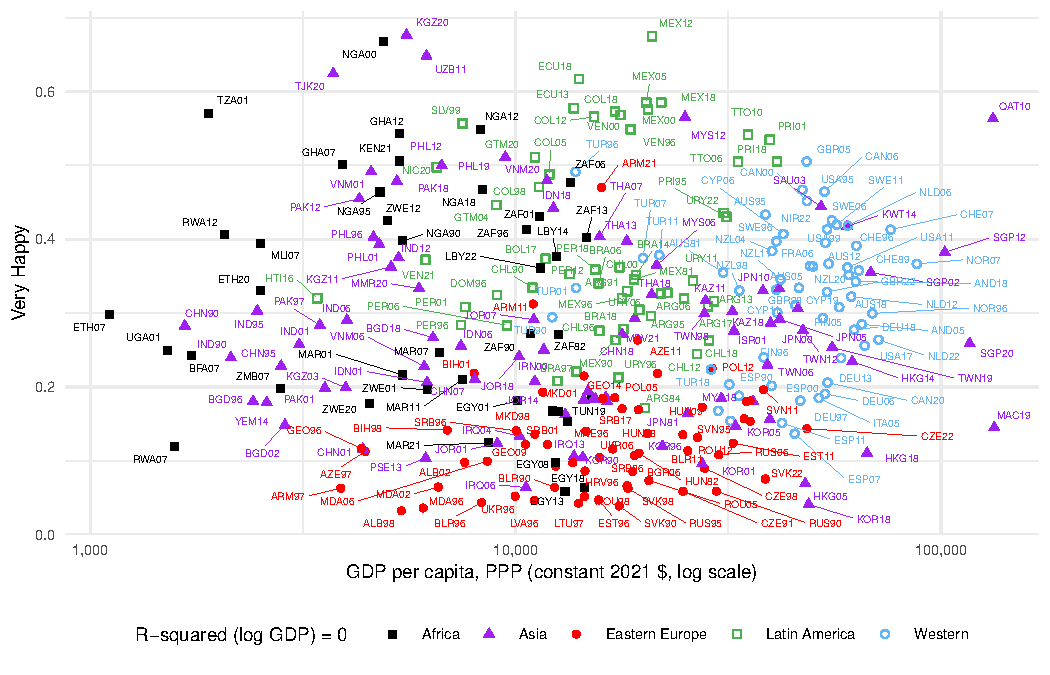
\includegraphics[width=.9\textwidth]{../figures/main/wvs_very_happy_vs_gdp_ppp.pdf}
    \caption{Share of \textit{Very happy} people vs.\ GDP per capita (PPP), WVS/EVS 1981--2023.}\label{fig:very_happy_gdp}
\end{figure}

\begin{figure}[htbp]
    \centering
    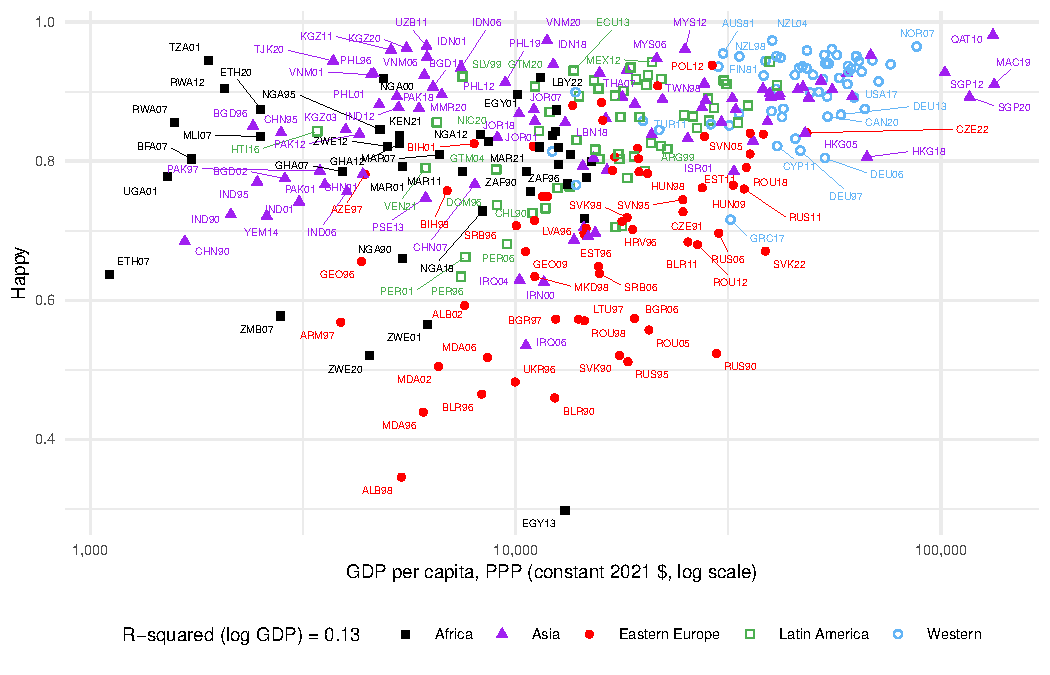
\includegraphics[width=.9\textwidth]{../figures/main/wvs_happy_vs_gdp_ppp.pdf}
    \caption{\textit{Happy} vs.\ GDP per capita (PPP), WVS/EVS 1981--2023.}\label{fig:happy_gdp}
\end{figure}

\begin{figure}[htbp]
    \centering
    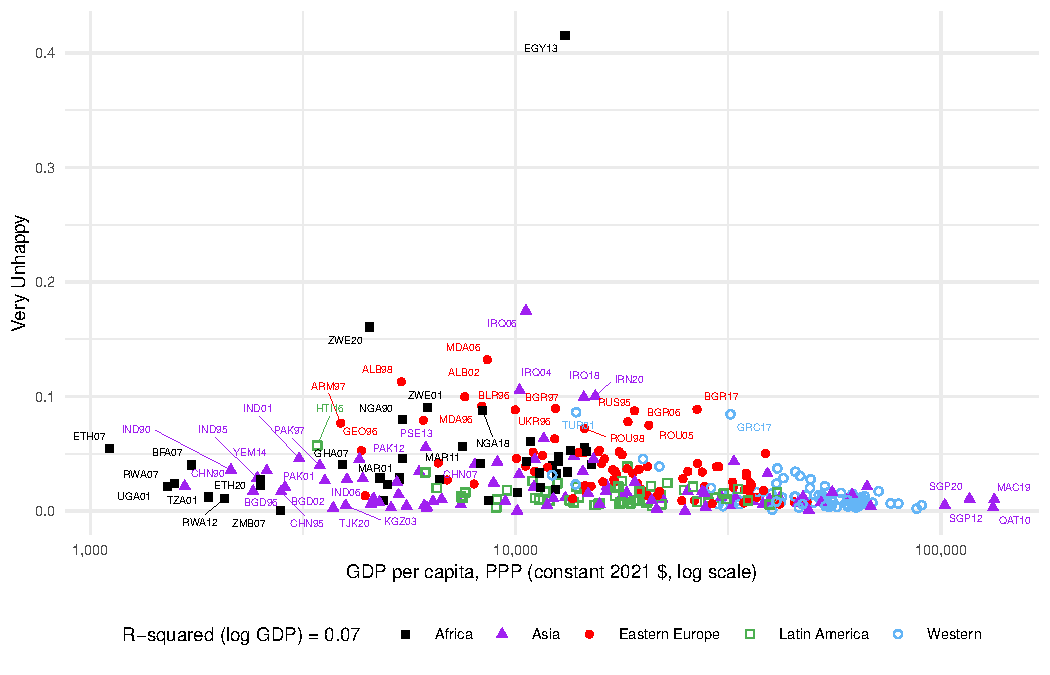
\includegraphics[width=.9\textwidth]{../figures/main/wvs_very_unhappy_vs_gdp_ppp.pdf}
    \caption{\textit{Very Unhappy} vs.\ GDP per capita (PPP), WVS/EVS 1981--2023.}\label{fig:very_unhappy_gdp}
    \begin{minipage}{.9\textwidth}\footnotesize \textit{Note:} Egypt 2013 (\veryUnhappyEGY\% of very unhappy people) is not shown, to keep the $y$-axis readable; the $R^2$ in the legend includes it.\end{minipage}
\end{figure}

\begin{figure}[htbp]
    \centering
    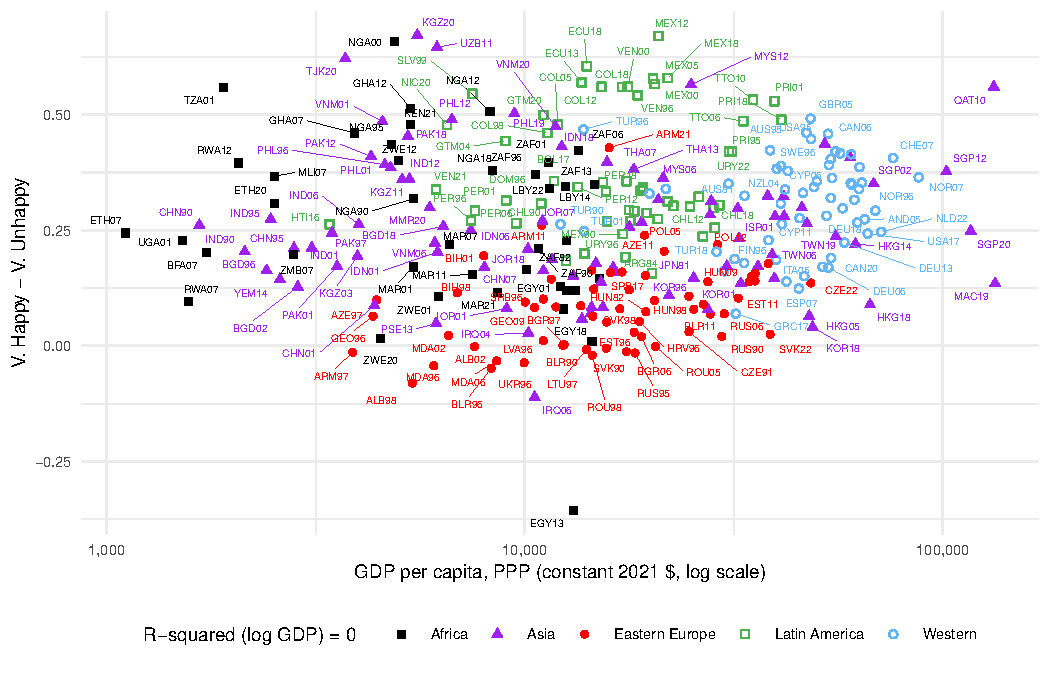
\includegraphics[width=.9\textwidth]{../figures/main/wvs_very_happy_minus_very_unhappy_vs_gdp_ppp.pdf}
    \caption{\textit{V.~Happy -- V.~Unhappy} vs.\ GDP per capita (PPP), WVS/EVS 1981--2023.}\label{fig:vhmvu_gdp}
\end{figure}

\begin{figure}[htbp]
    \centering
    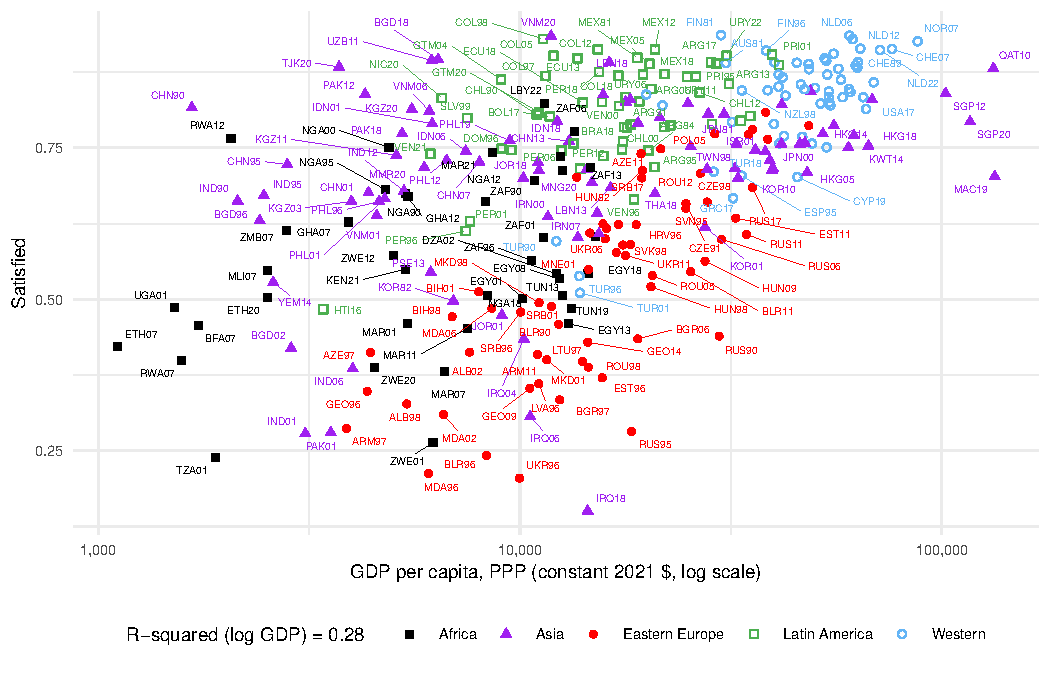
\includegraphics[width=.9\textwidth]{../figures/main/wvs_satisfied_vs_gdp_ppp.pdf}
    \caption{\textit{Satisfied} vs.\ GDP per capita (PPP), WVS/EVS 1981--2023.}\label{fig:satisfied_gdp}
\end{figure}

\begin{figure}[htbp]
    \centering
    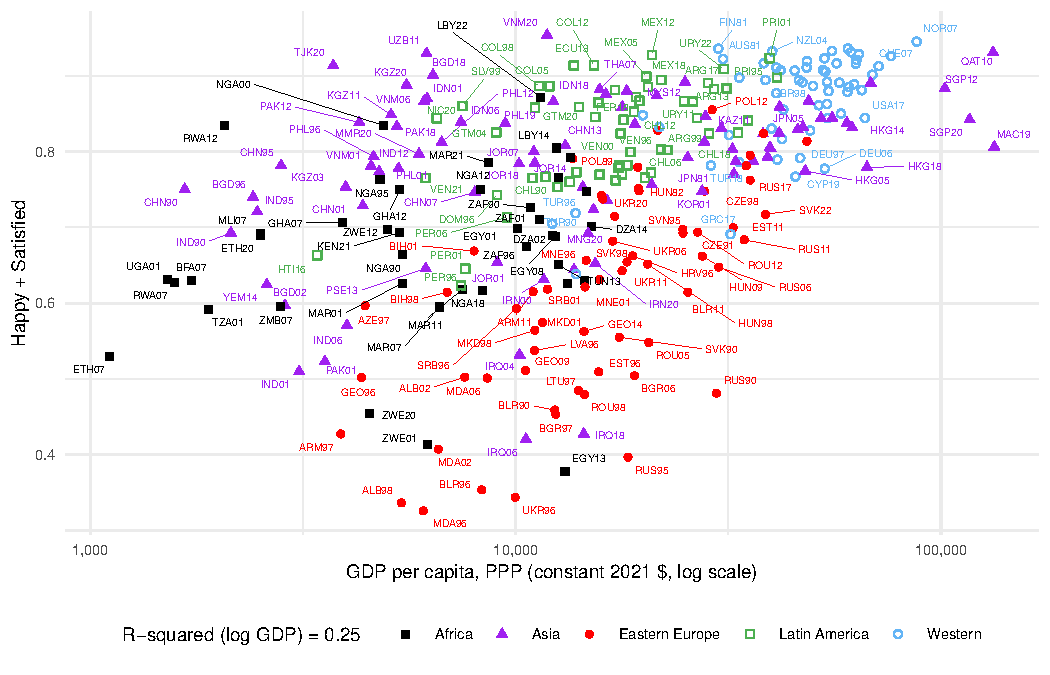
\includegraphics[width=.9\textwidth]{../figures/main/wvs_happiness_layard_vs_gdp_ppp.pdf}
    \caption{\textit{Happy + Satisfied} vs.\ GDP per capita (PPP), WVS/EVS 1981--2023.}\label{fig:layard_gdp}
\end{figure}

\begin{figure}[htbp]
    \centering
    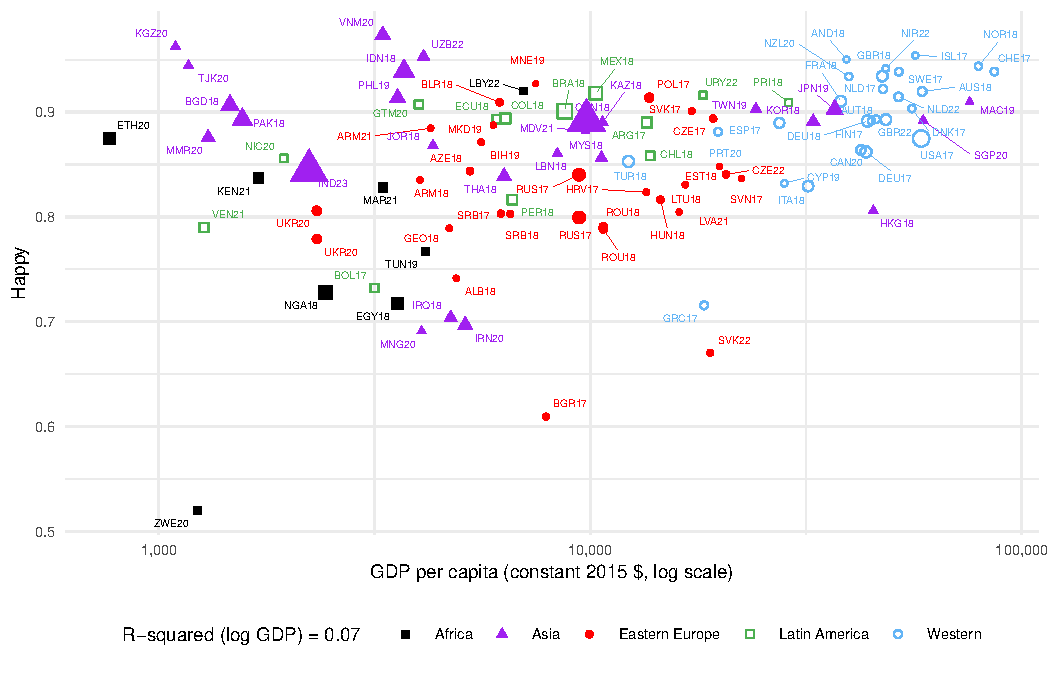
\includegraphics[width=.9\textwidth]{../figures/main/wvs_happy_vs_gdp_wave7_weighted.pdf}
    \caption{\textit{Happy} vs.\ GDP per capita (nominal), WVS/EVS wave 7 (2017--2023), weighted by population.}\label{fig:happy_gdp_w7_weighted}
    \begin{minipage}{.9\textwidth}\footnotesize \textit{Note:} Point size and regression weights proportional to population. \hfill(Back~to~Section~\ref{M-subsec:r2_income}.)\end{minipage}
\end{figure}

\clearpage
\bibliography{wellbeing}

\end{document}
